\documentclass{standalone}
\usepackage{tikz}
\usepackage{ctex,siunitx,upgreek}
\setCJKmainfont{Noto Serif CJK SC}
\usepackage{tkz-euclide}
\usepackage{amsmath,amsfonts,amssymb}
\usetikzlibrary{patterns, calc,3d}
\usetikzlibrary {decorations.pathmorphing,decorations.pathreplacing,decorations.shapes}
\tikzset{label style/.append style={font=\small}}
\begin{document}
\small
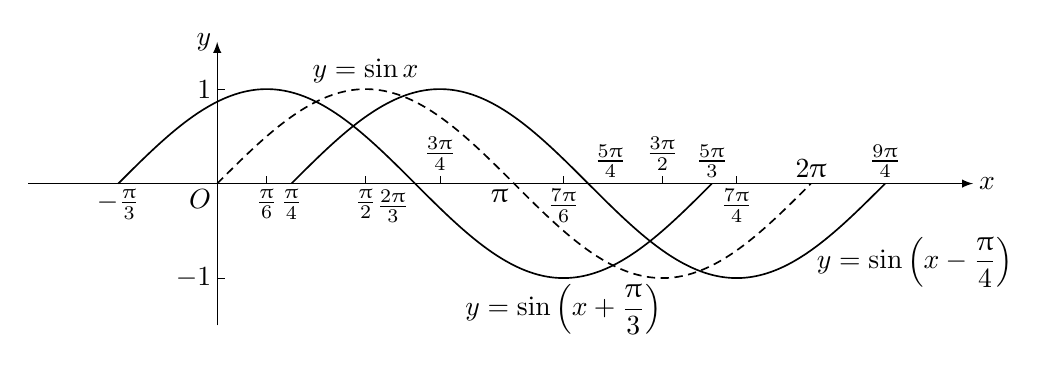
\begin{tikzpicture}[>=latex,scale=1.2,inner sep=2pt]
  \draw[->](-2,0)--(8,0)node[right]{$x$};
  \draw[->](0,-1.5)--(0,1.5)node[left]{$y$};
  \node at (0,0)[below left]{$O$};
  \draw[semithick,densely dashed,samples=200,domain=0:2*pi]plot(\x,{sin(\x r)});
  \draw[semithick,samples=200,domain=0:2*pi]plot(\x+0.25*pi,{sin(\x r)});
  \draw[semithick,samples=200,domain=0:2*pi]plot(\x-pi/3,{sin(\x r)});
  % \draw[semithick,samples=200,domain=0:pi]plot(\x,{sin(2*\x r)});
  \foreach \x in {-1,1} {\draw(0,\x)node[left]{$\x$}--++(0.08,0);}
  \node at (-pi/3,0)[below]{$-\frac\uppi3$};
  \node at (0.25*pi,0)[below]{$\frac\uppi4$};
  \node at (2.25*pi,0)[above]{$\frac{9\uppi}4$};
  \node at (pi,0)[below left]{$\uppi$};
  \node at (2*pi,0)[above]{$2\uppi$};
  \node at (2*pi/3,0)[below left]{$\frac{2\uppi}3$};
  \node at (5*pi/4,0)[above right]{$\frac{5\uppi}4$};
  \node at (5*pi/3,0)[above]{$\frac{5\uppi}3$};
  \draw[very thin](pi/6,0)node[below]{$\frac\uppi6$}--++(0,0.08);
  \draw[very thin](7*pi/6,0)node[below]{$\frac{7\uppi}6$}--++(0,0.08);
  \draw[very thin](7*pi/4,0)node[below]{$\frac{7\uppi}4$}--++(0,0.08);
  \draw[very thin](pi/2,0)node[below]{$\frac\uppi2$}--++(0,0.08);
  \draw[very thin](0.75*pi,0)--++(0,0.08)node[above]{$\frac{3\uppi}4$};
  \draw[very thin](1.5*pi,0)--++(0,0.08)node[above]{$\frac{3\uppi}2$};
  \node at (0.5*pi,1)[above]{$y=\sin x$};
  \node at (7*pi/6,-1)[below]{$y=\sin\left(x+\dfrac\uppi3\right)$};
  \node at (2*pi,-0.5)[below right]{$y=\sin\left(x-\dfrac\uppi4\right)$};
\end{tikzpicture}
\end{document}